\section{Use-Case Modellierung der untersuchten funktionalen Anforderungen}
\label{sec:use-case-modellierung}

Nachfolgend wird die ursprüngliche Anwendung funktional beschrieben, um daraus die Qualitätsanforderungen für die migrierte Anwendung abzuleiten. Durch das Testen auf die Qualitätsanforderungen soll untersucht werden, ob sich eine Veränderung im Nutzungsverhalten bei der Migration in die Cloud ergibt und ob das Migrationsziel erreicht wurde.

\subsection{Funktionale Beschreibung der bisherigen Anwendung}
Die Funktionalität der bisherigen Anwendung besteht darin, den Prozess der Rechnungsstellung zu automatisieren und somit management Aufwände zu reduzieren. Dazu besteht die Anwendung hauptsächlich aus drei Services, dem \textit{Collect Service}, dem \textit{Check Service} und dem dem \textit{Report Service}. Ausgeführt wird die Anwendung bisher auf einem lokalen System und greift über das lokale Verzeichnis mithilfe eines Desktop-Clients auf den online Speicherdienst \gls{Box} zu. Zur Ausführung der Anwendung wird eine Konfigurationsdatei benötigt, die alle notwendigen Pfade und Parameter enthält. In dem \gls{Box}-Verzeichnis liegen die \textit{\glspl{Timesheet}} der Mitarbeiter des Projektes und eine Projektmanagementdatei (PMO-File), die projektspezifische Informationen zum Projekt und den Mitarbeitern enthält.

Aufgabe des \textit{Collect Service} ist es, aus dem PMO-File oder einer alternativen Mitarbeiterliste alle, aktuell in dem Projekt aktiven Mitarbeiter zu ermitteln und die \textit{\glspl{Timesheet}} dieser in ein \textit{Collect}-Verzeichnis zu kopieren. Der \textit{Check Service} gleicht die von den Mitarbeitern manuell ausgefüllten \textit{\glspl{Timesheet}} mit den Daten aus einem Zeiterfassungstool ab und ermittelt, ob die Daten korrekt sind oder korrigiert diese automatisiert, sofern eine automatische Korrektur möglich ist. Abschließend werden im \textit{Report Service} aus Rechnungsdaten (Rechnungssumme, Leistungstext und Leistungsnachweise) für den konzerneigenen Rechnungsprozess ermittelt, erstellt und in einem Zielordner bereitgestellt. Da der Rechnungsprozess auf Einzelaufträgen basiert, wird die Information aus den \textit{\glspl{Timesheet}} detailliert auf die einzelnen Teilprojekten aufgeteilt.

In dieser Arbeit soll untersucht werden, ob sich eine Veränderung im Nutzungsverhalten durch die Migration in die Cloud ergibt und ob die Business-Logik entsprechend angepasst werden muss. \pagebreak

\subsection{Wie könnte ein Cloud Setup Aussehen?}
Durch die Migration in die Cloud ergeben sich viele Möglichkeiten für die Anwendung. Unter anderem bringt die Cloud-Migration \textit{\gls{Multi-Tenancy}}, also eine Mehrbenutzerfähigkeit mit sich, womit eine Instanz der Anwendung von mehreren Nutzern gleichzeitig verwendet werden kann. Die migrierte Anwendung muss entsprechend gestaltet sein, so dass die Fähigkeit gegeben ist, ohne dass diese sich beeinflussen oder behindern.

Um die Anwendung allgemein in die Cloud zu migrieren, könnte diese so wie sie ist mit \textit{Lift-and-Shift} in eine virtuelle Maschine kopiert werden und würde somit in der Cloud bereitgestellt. Dadurch könnte jedoch keine Aussage darüber getroffen werden, inwiefern die Anwendung oder ihre Architektur verändert werden muss, um als Cloud-nativen Anwendung die Vorteile der Cloud voll auszunutzen.

Um diese Anforderungen zu erfüllen, soll die existierende Anwendung zu einer Web-Anwendung umgeschrieben werden. Dadurch verändert sich die Art und Weise, wie die Use-Cases ausgeführt und angestoßen werden und wie die Anwendung benutzt wird. Diese Veränderungen werden am Beispiel der Migration des \textit{Collect Service} untersucht.

\subsection{Collect Service}
\textbf{Bisherige Verwendung:}

Der für den Prototypen ausgewählte Use-Case ist das ''Einsammeln'' der \textit{\glspl{Timesheet}}. Aus einer Konfigurationsdatei heraus soll festgelegt werden, für welches Projekt und welchen Zeitraum diese von dem Projektverzeichnis in ein temporäres Verzeichnis kopiert werden sollen. 

\textbf{Möglichkeiten einer Web-Anwendung:}

Durch die Migration in die Cloud und die Transformation zu einer Web-Anwendung werden die Funktionen der Anwendung zukünftig zum Beispiel über einen API-Endpunkt bereitgestellt oder die Ausführung dieser kann auch nach einem Zeitplan (Cron Job bzw. Batch Job) oder einem Trigger, wie das Hochladen einer neuen Konfigurationsdatei erfolgen. Auf die hierzu notwendigen technischen Veränderungen wird später in der Arbeit eingegangen. \pagebreak

\textbf{Use-Case Definition:}

Nachfolgend wird der Use-Case definiert, um im Anschluss an die Implementierung untersuchen zu können, ob dieser auch nach der Migration in die Cloud erfüllbar ist.

\begin{figure}[H]
    \centering
    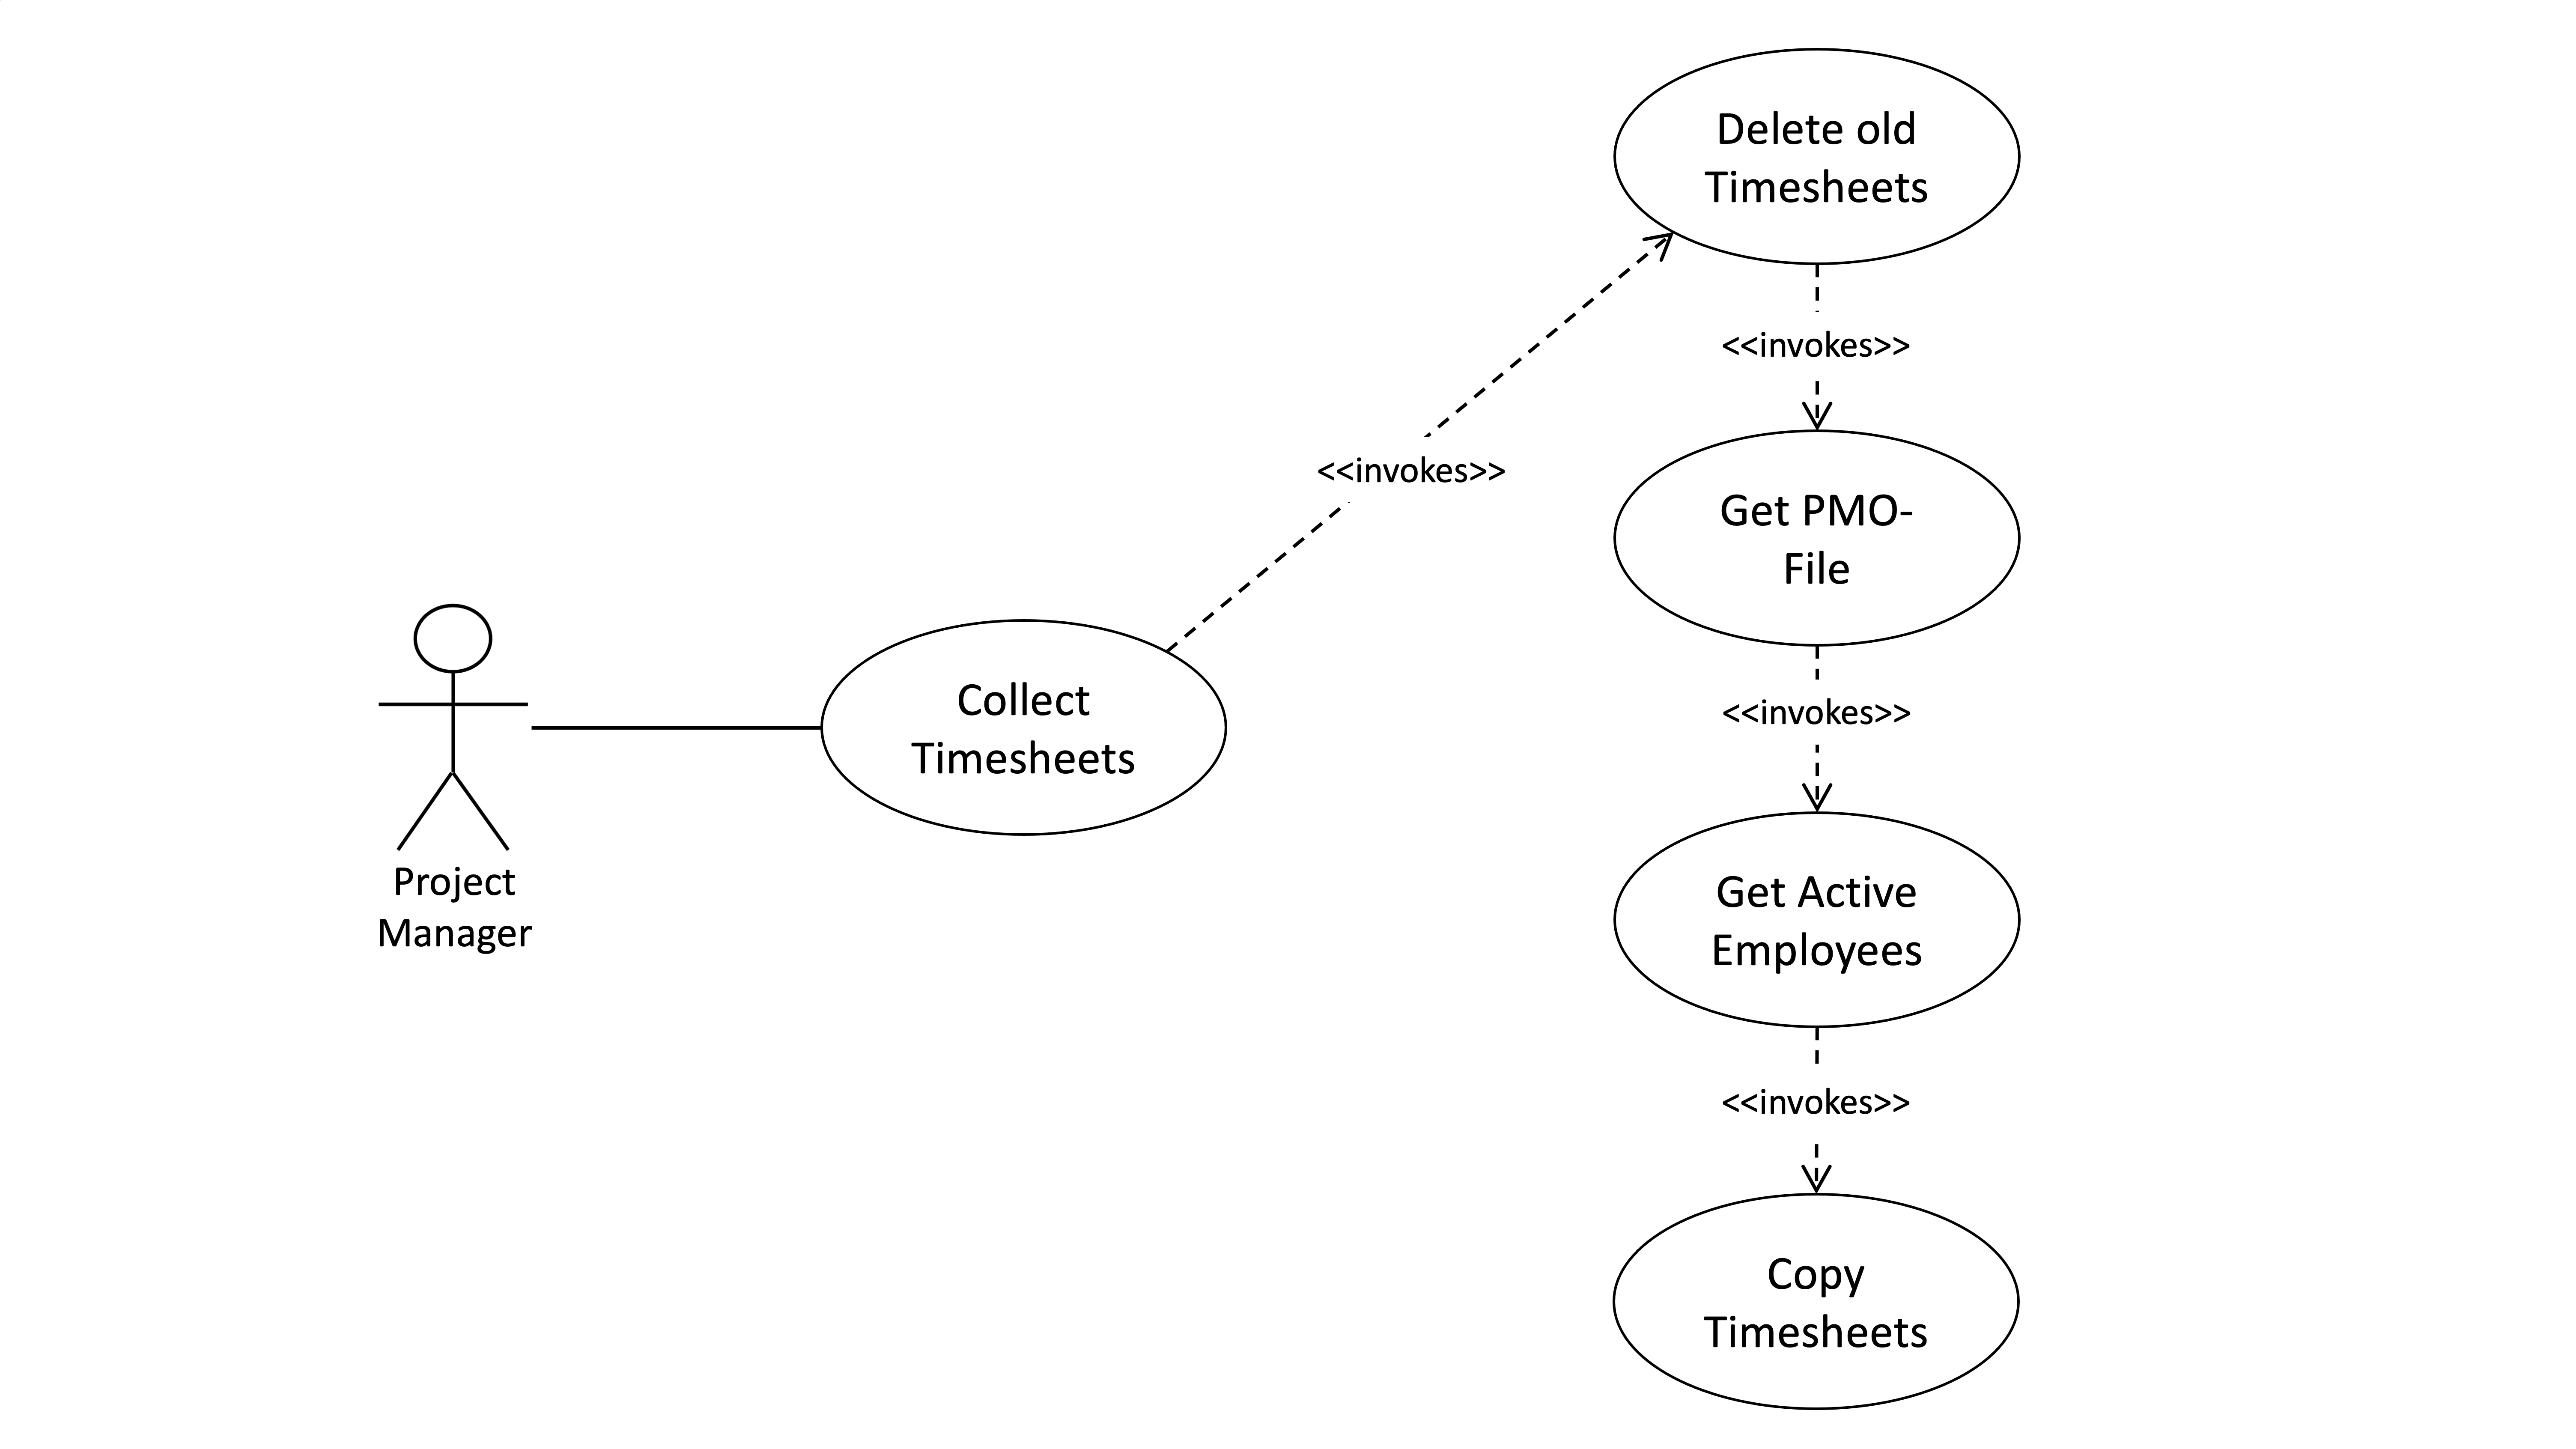
\includegraphics[width=\textwidth]{use-case-diagram.png}
    \caption{Use-Case Diagramm}
    \label{fig:use-case-diagram}
\end{figure}

Abbildung \ref{fig:use-case-diagram} stellt grafisch dar, welche Aufgaben der \textit{Collect Service} erfüllen muss und in welcher Reihenfolge diese ausgeführt werden. diese grundlegende Funktionsweise darf durch eine Cloud Migration nicht beeinträchtigt werden. Im folgenden wird dieser Use-Case nochmals formell beschrieben.

\begin{table}[H]
    \begin{tabular}[H]{|l|l|}
        \hline
        \multicolumn{2}{|l|}{\textbf{Anwendungsfall:} Einsammeln der \textit{\glspl{Timesheet}}} \\
        \hline
        \textbf{Kurzbeschreibung:} & \textit{\glspl{Timesheet}} aktiver Mitarbeiter in temporäres Verzeichnis kopieren \\
        \hline
        \multicolumn{2}{|l|}{\textbf{Normalverlauf}} \\
        \hline
        \multicolumn{2}{|l|}{1. Leeren des temporären Ordners} \\
        \multicolumn{2}{|l|}{2. PMO Datei finden und laden} \\
        \multicolumn{2}{|l|}{3. Aktive Mitarbeiter aus PMO Datei lesen} \\
        \multicolumn{2}{|l|}{4. \textit{\glspl{Timesheet}} der aktiven Mitarbeiter kopieren} \\
        \hline
        \multicolumn{2}{|l|}{\textbf{Alternativablauf}} \\
        \hline
        \multicolumn{2}{|l|}{N/A} \\
        \multicolumn{2}{|l|}{\textbf{Qualitätsanforderungen}} \\
        \hline
        \multicolumn{2}{|l|}{1. Für jeden aktiven Mitarbeiter soll ein \textit{\gls{Timesheet}} im temporären Ordner liegen} \\
        \multicolumn{2}{|l|}{2. Die \textit{\glspl{Timesheet}} sollen unverändert sein (Dateiname, Inhalt)} \\
        \multicolumn{2}{|l|}{3. Eigener Zielordner pro Monat zur Vermeidung von Vermischungen} \\
        \multicolumn{2}{|l|}{4. Die \textit{\gls{Timesheet}} Größe kann variieren -> keine Limitierungen} \\
        \multicolumn{2}{|l|}{5. Es darf keine Kompression mit Formatänderung eingesetzt werden} \\
        \multicolumn{2}{|l|}{6. Ein Logfile soll Erfolg und Misserfolg von Kopiervorgängen enthalten} \\
        \multicolumn{2}{|l|}{7. Fehlersituationen auf einzelnen Dateien dürfen den Ablauf nicht unterbrechen} \\
        \multicolumn{2}{|l|}{8. Root-Verzeichnisse für Ziel und Quelle müssen konfigurierbar sein} \\
        \hline
    \end{tabular}
    \caption{Anwendungsfall: Einsammeln der \textit{\glspl{Timesheet}}}
    \label{tab:use-case-analyse-timesheets}
\end{table}

Anschließend an diesen Prozess würden die weiteren Services der Gesamtanwendung folgen, welche jedoch nicht näher in dieser Arbeit untersucht werden.